
\documentclass[12pt]{article}

\usepackage{graphicx}
\graphicspath{ {./images/} }

\usepackage{epsfig}
\usepackage{amsmath,amsthm}
\usepackage{listings}


\newtheorem{lemma}{Lemma}
\newtheorem{theorem}{Theorem}


\usepackage{titlesec}
\titleformat{\section}
{\normalfont\Large\bfseries}{Question~\thesection:}{1em}{}

\newlength{\toppush}
\setlength{\toppush}{2\headheight}
\addtolength{\toppush}{\headsep}


\def\subjnum{Comp 170}
\def\subjname{Computation Theory}


\def\doheading#1#2#3{\vfill\eject\vspace*{-\toppush}%
  \vbox{\hbox to\textwidth{{\bf} \subjnum: \subjname \hfil Erli Cai}%
    \hbox to\textwidth{{\bf} Tufts University, Fall 2020 \hfil#3\strut}%
    \hrule}}


\newcommand{\htitle}[1]{\vspace*{1.25ex plus 1ex minus 0ex}%
\begin{center}
{\large\bf #1}
\end{center}} 



\begin{document}
\doheading{2}{title}{Homework 04}

\setlength\parindent{0pt}

\section{Expressions to Machines}
(a)\\ 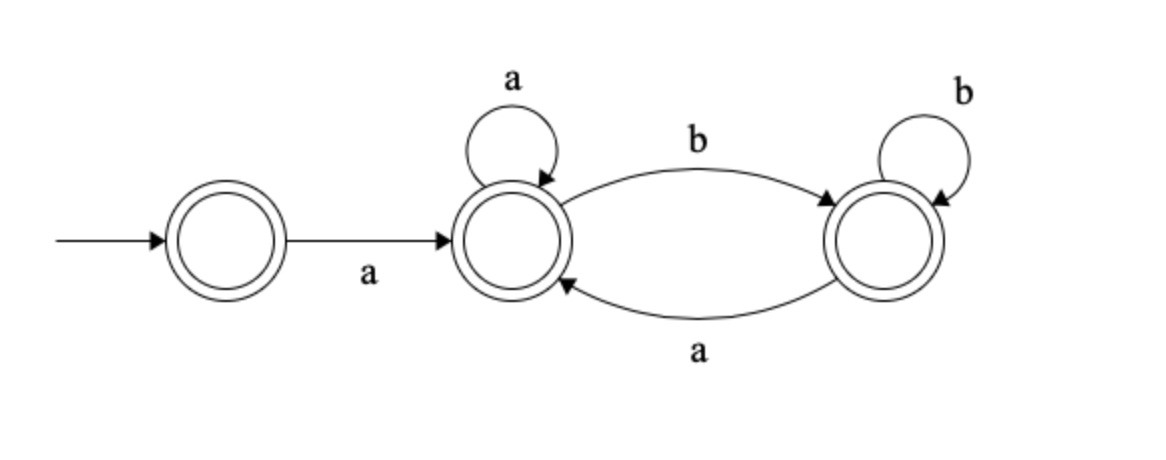
\includegraphics[scale = 0.5]{1}

(b)\\ 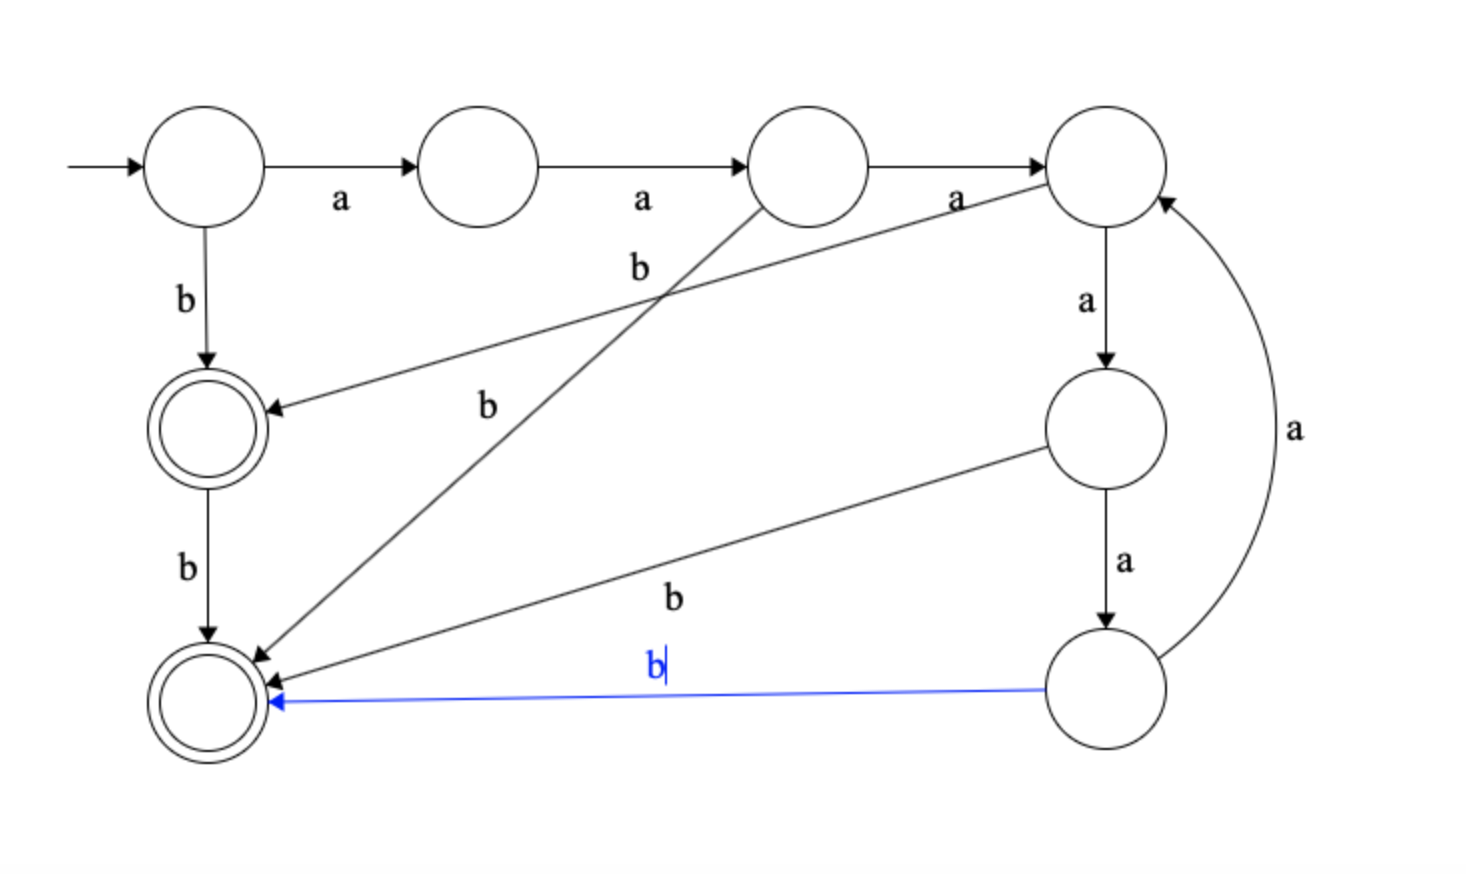
\includegraphics[scale = 0.5]{2}
\pagebreak

(c)\\ 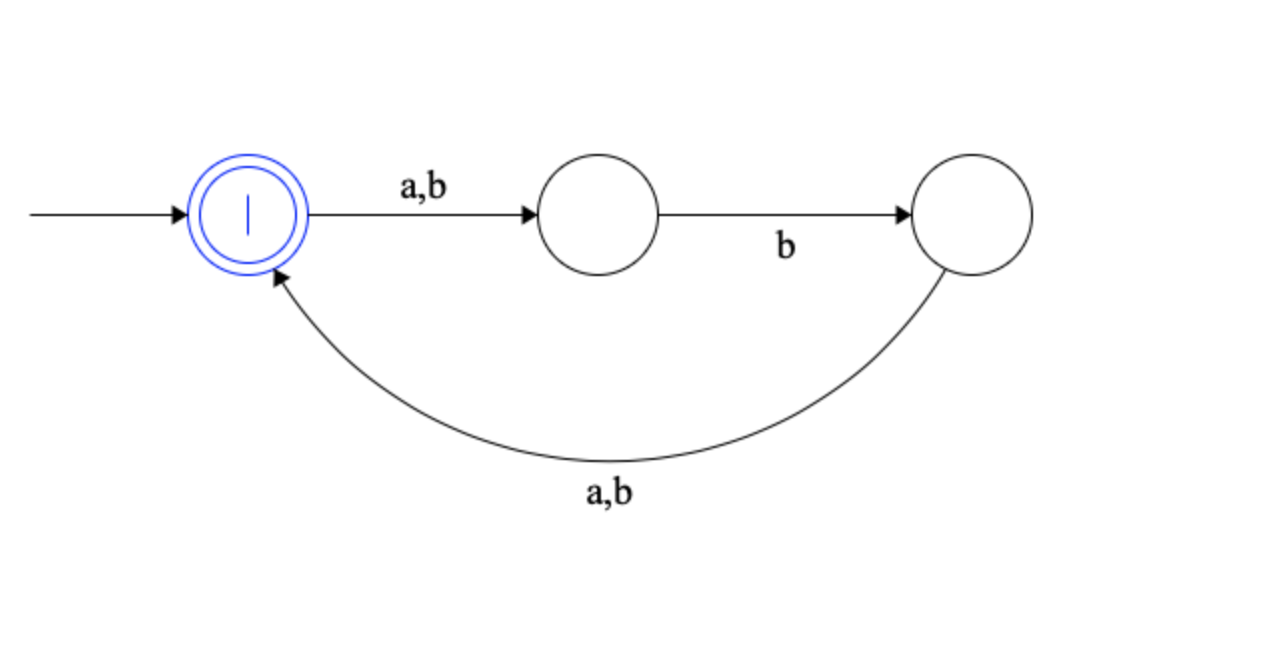
\includegraphics[scale = 0.5]{3}
\pagebreak

\section{Just One Difference}
\begin{center}
\begin{tabular}{rll}
$L_1$ & = & $\{xy~|~ x,y \in \{a,b\}^*, \#a(x) = \#b(y)\}$\\
$L_2$ & = & $\{xcy~|~ x,y \in \{a,b\}^*, \#a(x) = \#b(y)\}$
\end{tabular}
\end{center}

$L_1$ is regular while $L_2$ is not.\\

$L_1$ = $\{a, b\}^*$ \\
Therefore, $L_1$ is regular\\


Now, prove $L_2$ is not regular.\\
For any given $p \ge 1$\\
let $w = a^pcb^p$\\
For any ways to writes w as $ w = xyz$ with $|xy| \le p$, $|y| \ge 1$, \\
y must be a string of a(s) and have at least one a, $y = a^k$, $ 1\le k\le q$. 
Therefore, if we pump y twice we get $a^{k+q}cb^q$, which is not an element of $L_2$.
In conclusion, $L_2$ is not regular.

\pagebreak



\section{Context Free Grammars}

a.  $S \rightarrow  aS | bS | \epsilon $\\

b. First proving that $L(G) \subseteq A$\\
Base Case:\\
$S \xrightarrow{1} \epsilon$ If $x = y =\epsilon$,  then $\#a(x) = \#b(y)$ , so $\epsilon \in A$ \\


For the inductive step, suppose the claim is true for some $i \ge 1$. That is, suppose we know that for
any $m\in\Sigma$, if $S \xrightarrow{i} m$ then $m\in A$. Now consider $n\in\Sigma$ such that 
$S \xrightarrow{i+1} n$ ;we want to show that $n \in A$ . There are four cases:

1) $S\xrightarrow{1} aS  \xrightarrow{s} n$. Then n = am for some $m\in \Sigma^*$. By induction hypothesis, m = xy where $\#a(x) = \#b(y)$ If we let $x' =$ a followed by x except last charter in x and $y' = $ last character in x followed by y, \\
either this character is a, then $\#a(x') =1+ \#a(x) - 1 = \#a(x)$ and  $\#b(y') = 0+  \#b(y) = \#b(y)$\\
or this character is b, then $\#a(x') = \#a(x) - 1 $ and  $\#b(y') = \#b(y)  - 1 $\\
Either way, we still get $\# a(x') = \# b(y')$, so $n \in A$

2) $S\xrightarrow{1} bS  \xrightarrow{s} n$. Then n = bm for some $m\in \Sigma^*$. By induction hypothesis, m = xy where $\#a(x) = \#b(y)$ If we let $x' =$ a followed by x and $y' = $y, \\
then $\#a(x') = \#a(x)  $ and  $\#b(y') = \#b(y)  $\\we still get $\# a(x') = \# b(y')$, so $n \in A$\\
By mathematical induction,  $n \in A$. Thus $L(G) \subseteq A$\\

Now proving that $A \subseteq L(G)$\\
Base case: $m = \epsilon$. Then $S\xrightarrow{1} \epsilon$ is the derivation for m.
Induction Hypothesis: For the inductive step, consider a palindrome n with $|n| \ge 1$ and suppose the claim is true for all shorter n. 
We must have either n = am or n = bm for some m.
If n= am then we can use derivation $S \xrightarrow{1} aS \xrightarrow{*} am =n \ $
If n = bm then we can use derivation $S \xrightarrow{1} bS \xrightarrow{*} bm =n \ $
By mathematical induction, $n\in L(G)$. Thus, $A \subseteq L(G)$\\



\end{document}


